\section{连续LTI系统的卷积模型}

本节讨论LTI系统在连续时域的卷积模型。

本节要点:
\begin{itemize}
    \item 理解卷积积分的概念;
    \item 掌握LTI系统的卷积模型;
    \item 熟悉卷积模型对系统的要求。
\end{itemize}

%============================================================
\subsection{卷积积分和卷积模型}

\begin{definition}[冲激响应]
我们称单位冲激信号$\delta \left( t \right) $经过系统后的输出称为{\bf 单位冲激响应},简称{\bf 冲激响应},记为$h\left( t \right) $。
\end{definition}

\begin{definition}[卷积积分]
对于两个连续函数$a\left( t \right) ,b\left( t \right) ,t\in \mathbb{R} $,如果广义积分$\int_{-\infty}^{+\infty}{a\left( \tau \right) b\left( t-\tau \right) d\tau}$收敛,则称该积分为{\bf $a\left( t \right) ,b\left( t \right) $的卷积积分}(convolution integral),记为$a\left( t \right) \ast b\left( t \right) $,即:
\[
a\left( t \right) \ast b\left( t \right) =\int_{-\infty}^{+\infty}{a\left( \tau \right) b\left( t-\tau \right) d\tau}
\]
\end{definition}

{\bf 连续LTI系统的卷积模型}:若一LTI系统符合因果律且零状态,系统的冲激响应为$h\left( t \right) $,当$h\left( t \right) $和输入信号$x\left( t \right) $在$\left[ 0,t \right] $绝对可积:
\begin{align*}
&\int_0^t{\left| x\left( \tau \right) \right|d\tau}<\infty \\
&\int_0^t{\left| h\left( \tau \right) \right|d\tau}<\infty
\end{align*}
则该系统对任何输入信号的响应可以表示为输入信号$x\left( t \right) $和冲激响应$h\left( t \right) $的卷积,即:
\[
y\left( t \right) =x\left( t \right) \ast h\left( t \right) =\begin{cases}
	0 &t<0\\
	\int_0^t{x\left( \tau \right) h\left( t-\tau \right) d\tau} &t\geqslant 0\\
\end{cases}
\]
该表达式称为{\bf 系统的卷积模型}。

%============================================================
\subsection{微分方程模型和卷积模型}

至此,对于一个LTI系统,我么可以用微分方程和卷积两种方法描述:
\begin{align*}
&y^{\left( n \right)}\left( t \right) +\sum_{i=0}^{n-1}{A_iy^{\left( i \right)}\left( t \right)}=\sum_{i=0}^m{B_ix^{\left( i \right)}\left( t \right)} \\
&y\left( t \right) =x\left( t \right) \ast h\left( t \right)
\end{align*}
两种模型都要求系统是LTI,区别在于:
\begin{itemize}
    \item 微分方程要求是有限维度,用系数$A_0,A_1,\cdots ,A_{n-1},B_0,B_1,\cdots ,B_m$描述系统,不同系统的区别就在于不同的系数。
    \item 卷积要求是符合因果律,再加上$x\left( t \right) ,h\left( t \right) $绝对可积,用冲激响应$h\left( t \right) $描述系统,不同系统的区别在于不同的$h\left( t \right) $。
\end{itemize}
两个模型中,微分方程对应着卷积运算,微分方程的系数对应着冲激响应。

%============================================================
\subsection{一阶微分方程系统的零状态冲激响应}

对于一阶微分方程的系统$\frac{dy\left( t \right)}{dt}+Py\left( t \right) =Qx\left( t \right) $,考虑零状态($y\left( 0 \right) =0$)响应:
\[
y\left( t \right) =e^{-Pt}\left[ e^{-Pt_0}y\left( t_0 \right) +Q\int_{t_0}^t{e^{-P\tau}x\left( \tau \right) d\tau} \right] =e^{-Pt}\left[ Q\int_0^t{e^{-P\tau}x\left( \tau \right) d\tau} \right]
\]
冲激响应:
\[
h\left( t \right) =\left. y \right|_{x=\delta}=e^{-Pt}\left[ Q\int_0^t{e^{-P\tau}\delta \left( \tau \right) d\tau} \right] =Qe^{-Pt}
\]
可见,零状态的一阶微分系统有着一样的冲激响应。

%============================================================
\subsection{例RC电路}

\begin{example}
依然以RC电路为例,(1)试从微分方程推导系统的冲激响应,(2)写出系统的卷积模型,(3)如果输入信号为$x\left( t \right) =1$,求解输出。
\end{example}
\begin{figure}[h]
\centering
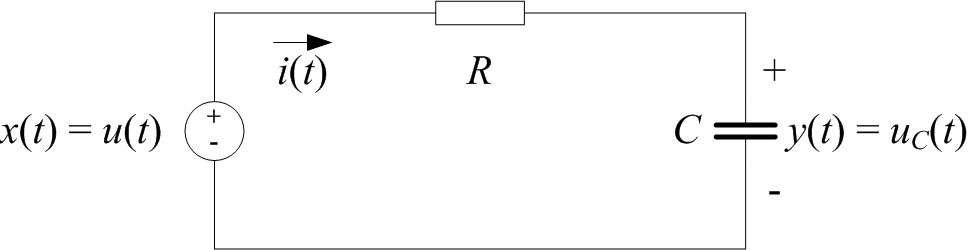
\includegraphics[height=2cm]{1.5.1-1.png}
\end{figure}


(1)令输入信号为冲激函数,求解得到冲激响应:
\begin{align*}
&\because \frac{dy}{dt}+\frac{1}{RC}y=\frac{1}{RC}x \qquad \begin{cases}
	x\left( t \right) =\delta \left( t \right)\\
	y\left( 0^- \right) =0\\
\end{cases} \\
&\therefore h\left( t \right) =e^{-Pt}\left[ Q\int_0^t{e^{-P\tau}\delta \left( \tau \right) d\tau} \right] =\frac{1}{RC}e^{-\frac{t}{RC}}
\end{align*}

(2)系统的卷积模型:
\[
y\left( t \right) =x\left( t \right) \ast h\left( t \right) =\int_0^t{x\left( \tau \right) \frac{1}{RC}e^{-\frac{t-\tau}{RC}}d\tau} \qquad t\geqslant 0
\]

(3)将输入信号带入,计算得到输出:
\[
y\left( t \right) =\int_0^t{\frac{1}{RC}e^{-\frac{t-\tau}{RC}}d\tau}=1-e^{-\frac{t}{RC}} \qquad t\geqslant 0
\]




